\section{System Design}
\label{sec:design}
The architecture connects two configurable sides of an industrial deployment:
an agent collaboration runtime and a production-scene configuration. The
runtime supplies task context and scoped operations; scene configuration maps
process semantics to acquisition and control nodes, drivers, targets, and
guards. Named operations connect these sides to shared dispatch and governed
device access. The design separates task execution from operation dispatch and
keeps command receipts distinct from measured process responses.

\begin{figure*}[!t]
\centering
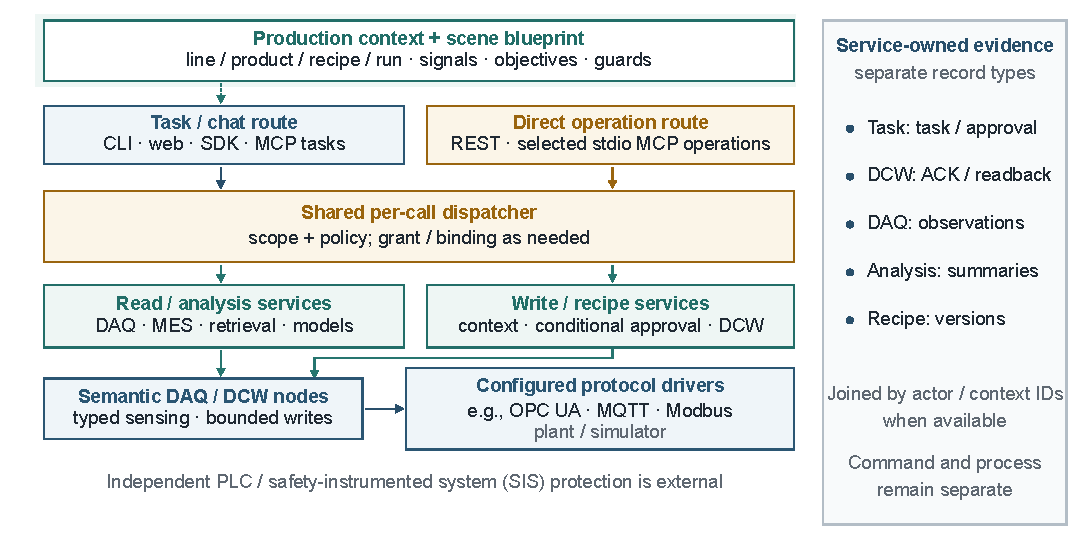
\includegraphics[width=\textwidth]{resources/fig-architecture-2026-9pt.pdf}
\caption{Architecture and record ownership. Task/chat routes enter the
collaboration runtime; direct REST and stdio-MCP calls enter shared dispatch
checks without creating a task. One dashed link marks configuration. Write
routes apply interval admission and, when configured, approval; recipe dispatch omits the
previous-recipe window. The shared dispatcher always
checks scope and channel policy, with grant and resource-binding checks applied
when required by the operation. Owning services retain distinct records; plant
controllers and safety systems retain equipment interlocks.}
\label{fig:arch}
\end{figure*}

\subsection{Design Rationale and Requirements}
\label{sec:principles}
Three design requirements follow from the deployment problem. Scene
configuration must preserve process meaning while mapping signals and controls
to heterogeneous drivers. Harness variation must not change the operation
contract. Each write must also be checked against current authority and
process limits, with its command receipt distinguishable from later process
measurements. The architecture addresses these requirements through
scene-bound data-acquisition and write-control nodes, registered harness
adapters, a shared dispatcher, and service-owned records. The registry
provides an extension point for additional agent engines and protocol drivers;
the experiment evaluates only the configured simulator paths described in
Section~\ref{sec:eval}. Tool visibility alone does not authorize a write:
actuator operations pass through the shared write-admission point.

Commissioning associates the line with products, recipes, active-run rules,
signal meanings, units, driver mappings, and admissible limits. At runtime,
the context builder assembles the active line--product--recipe--run state and
relevant process summaries for each agent turn. An operation handler resolves
live state again before dispatch, so the prompt context informs a proposal but
does not substitute for current authorization or admission checks. Direct
operations resolve the current context at invocation without creating a task.

\subsection{Layered Architecture}
\label{sec:layers}
\label{sec:arch}
Fig.~\ref{fig:arch} summarizes the access routes, shared dispatch path,
production services, semantic I/O, configured drivers, and service ownership
of records. Task and chat routes enter the collaboration runtime, which
contains workspaces, channels, task queues, shared memory, mailboxes, task
templates, and harness adapters. A \emph{task route} is an execution path
through this runtime; a \emph{harness adapter} connects an agent engine to its
task interface. Multiple registered agents can participate through shared
tasks and channel context, with each agent's available tools constrained by
its binding and channel policy. Direct REST tool
calls and the stdio MCP operation bridge bypass task execution in that band
(the upper-right direct-operation entry in
Fig.~\ref{fig:arch}) and enter the shared governance block without creating a
task or starting a harness turn; MCP management and task methods remain on
their service routes. Direct calls resolve current route state at invocation,
without an agent-turn prompt or a task record.
The governance block projects the operation catalog and applies the per-call
checks. Write handlers apply admission limits and request approval when the
operation and its configuration require it. The
context block supplies the active line--product--recipe--run tuple to the gate
and scene maps, objectives, and guards to the handlers. The dashed link from
that block in Fig.~\ref{fig:arch} marks this configuration relationship; the
runtime assembles prompt-time context from the same records. The service band,
behind a route-handler interface that selects an adapter, provides data
acquisition, write control, analysis, retrieval, and optional model services.
Field I/O resolves semantic nodes to built-in or plugin drivers for a plant or
simulator. Services retain task, command, observation, and configuration
records separately and associate them with actor and production context.

\subsection{Cross-Module Execution Flow}
\label{sec:executionflow}
Fig.~\ref{fig:runtime} summarizes a task turn from entry through operation
execution, with route-specific evidence retained by owning services. Registered
harness adapters receive a scoped tool catalog during setup and supported
registry refreshes; the runtime assembles prompt-time production context from
current records for each agent turn. For each returned tool call, the shared
dispatcher rechecks invocation scope, channel policy, and applicable grant and
binding conditions before handler selection. The selected handler
then applies route-specific guards, active-run checks, approval
revalidation, and device-I/O steps as applicable. Command receipts and later
process observations remain distinct records.

For an industrial operation $u$ by agent $a$ in channel $c$, define the
shared dispatch condition as
\begin{equation}
\mathcal{A}(a,c,u)=\bigwedge_{X\in\mathcal{C}(u)}X(a,c,u),
\label{eq:dispatch-contract}
\end{equation}
where $S$, $P$, $G$, and $B$ denote invocation scope, current channel policy,
applicable industrial grant, and the agent's binding to referenced resources,
respectively. $\mathcal{C}(u)\subseteq\{S,P,G,B\}$ is the set of predicates
declared for operation $u$; it always contains $S$ and $P$. The grant predicate
$G$ is included when the resolved channel, target line, and owner/grant policy
require it; explicit exemptions omit it. The binding predicate $B$ is included
when the operation declares resource references. A declared no-reference
operation omits $B$. Each included check must pass before
handler selection. The policy predicate includes channel tool selection,
profile, and duty-separation checks where configured. Once these predicates
pass, the selected route applies its guards, active-run checks, admission
limits, and any required approval. When approval is required, the handler
revalidates its context before device dispatch.

For direct REST invocation, the service establishes $a$ and $c$ before applying
these checks: an agent token must match the requested agent identifier, or an
authenticated user must be the channel owner or an administrator. The manager
loads the channel-agent record and rechecks scope and policy; applicable grant
and binding checks follow. Handlers resolve live
production state from request identifiers and owning services.

Fig.~\ref{fig:execution} gives reference pseudocode summarizing the
registered-harness task path. Direct REST tool invocation
bypasses the task runtime and harness but enters the same shared dispatcher.
Route-specific timing, approval, and evidence rules are detailed in
Section~\ref{sec:modules}.

\begin{figure*}[!t]
\centering
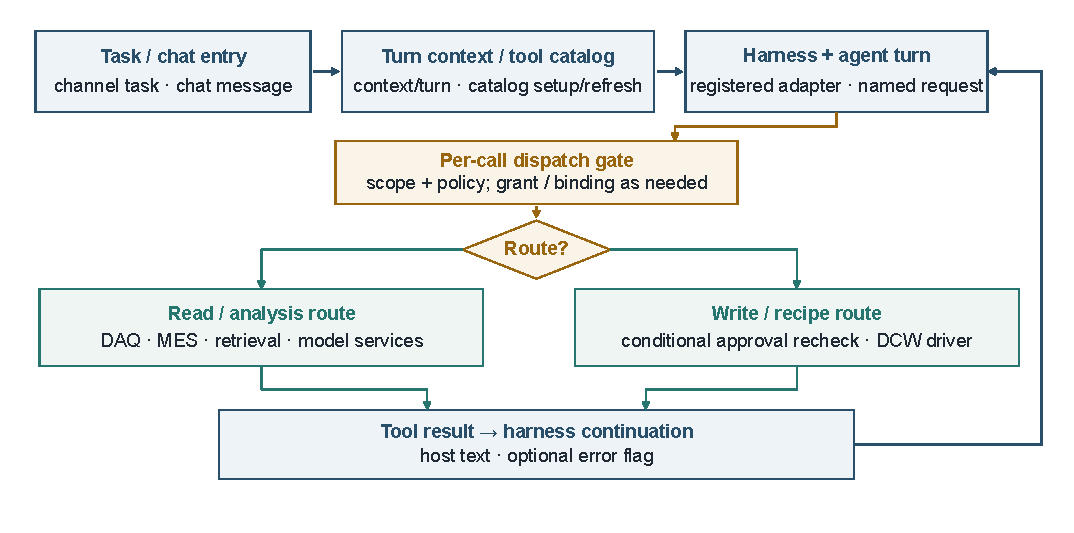
\includegraphics[width=\textwidth]{resources/fig-runtime-2026-9pt.pdf}
\caption{Registered-harness task flow. The runtime invokes the adapter with a
scoped catalog. Scope and channel policy are checked for every call; grant
applies to non-exempt industrial operations, and binding applies when resource
references are declared. Failed checks return tool errors. The read path
retrieves data. The write path applies route guards, conditional approval and
its context revalidation, write admission, and receipt grading; a later process
observation is separate. Results return to the harness. Device-level interlocks remain
with the configured plant-control layer.}
\label{fig:runtime}
\end{figure*}

\begin{figure}[!t]
\centering
\begin{algorithmic}[1]
\Require task $q$, channel $c$, bound agent $a$, registered scoped catalog $T$
\Ensure task result; any retained evidence remains with its owning service
\State $x_t \gets \Call{ResolvePromptContext}{c,q}$
\State $m \gets \Call{RetrieveMemory}{q}$
\State $p \gets \Call{AssemblePrompt}{q,x_t,m}$
\State $h \gets \Call{InvokeRegisteredHarness}{a,p,T}$
\ForAll{tool request $u$ returned by $h$}
  \State $g \gets \Call{CheckScopeAndChannelPolicy}{a,c,u}$
  \If{\textbf{not} $g$}
    \State \Call{EmitToolErrorToHarness}{h,u}; \textbf{continue}
  \EndIf
  \If{$u$ is an industrial operation}
    \State $v \gets \Call{CheckApplicableGrantBinding}{a,u}$
    \If{\textbf{not} $v$}
      \State \Call{EmitToolErrorToHarness}{h,u}
      \State \textbf{continue}
    \EndIf
  \EndIf
  \State $k \gets \Call{SelectHandler}{u}$
  \State $r \gets \Call{ExecuteRouteHandler}{k,a,c,u}$
  \Comment{handler resolves live state and may persist route-specific records}
  \State \Call{EmitDeclaredToolResultToHarness}{h,r}
\EndFor
\State \Return task state and tool results
\end{algorithmic}
\caption{Reference pseudocode for the registered-harness task path. Direct
operation calls use the shared dispatcher from their own entry point. Each
route persists records through its owning service and returns its declared
response to its caller; task-route results return to the harness.}
\label{fig:execution}
\end{figure}
